\chapter{Analýza a návrh systému}
V této kapitole je popsán proces transformace teoretických poznatků do konkrétního softwarového návrhu. Návrh se zaměřuje na vytvoření modulárního systému pro generování instancí problému obchodního cestujícího s využitím externích geolokačních dat %%\cite{20}.

\section{Analýza požadavků}
Na základě zadání práce byly definovány klíčové požadavky, které jsou rozděleny na funkční (definující chování systému) a nefunkční (definující vlastnosti a omezení).

\subsection{Funkční požadavky}
\begin{table}[ht]
\centering
\begin{tabular}{|l|p{10cm}|}
\hline
\textbf{ID} & \textbf{Popis požadavku} \\ \hline
F1 & Systém umožní import seznamu lokalit (názvy měst, GPS souřadnice) z externího souboru. \\ \hline
F2 & Systém provede výpočet matice vzdáleností a časů pomocí mapového API nebo lokálního modelu %%\cite{20, 23}. 
\\ \hline
F3 & Systém umožní export vygenerované instance do formátů standardizovaného formátu TSPLIB %%\cite{26}. 
\\ \hline
F4 & Systém zajistí vizualizaci vstupních bodů a vypočtené optimální trasy nad mapovým podkladem %%\cite{20}. 
\\ \hline
% F5 & Systém umožní konfiguraci parametrů generování (např. typ dopravy: auto, pěší). \\ \hline
\end{tabular}
\caption{Funkční požadavky systému}
\end{table}

\clearpage

\subsection{Nefunkční požadavky}
\begin{itemize}
    \item Vzhledem k výpočetní náročnosti analýzy větších instancí TSP využívá aplikace vícevláknové zpracování v prostředí Qt. Výpočetní a síťově náročné kroky jsou přesunuty mimo hlavní vlákno uživatelského rozhraní, což udržuje aplikaci plynule ovladatelnou
    \item \textbf{Portabilita:} Systém bude implementován, jak již bylo zmíněno výše, v jazyce Python, což zajistí multiplatformní běh (Windows, Linux, macOS)
    \item \textbf{Modularita:} Architektura odděluje vrstvu rozhraní, jádro optimalizace, routovací vrstvu, správu stavu a I/O, takže lze systém postupně rozšiřovat bez zásahů do všech částí současně
    \item \textbf{Licenční čistota:} Systém bude prioritně využívat open-source řešení (OSRM, OSM) nevyžadující placené API klíče %%\cite{23}.
    \item \textbf{Uživatelské rozhraní:} Aplikace bude poskytovat přehledné grafické rozhraní pro vizualizaci
\end{itemize}

\section{UML analýza}
Pro formální zachycení struktury, interakcí a dynamického chování navrženého systému byly využity standardizované diagramy jazyka UML. Tato vizualizace slouží k dekompozici komplexních procesů generování instancí a k definici jasných rozhraní mezi výpočetním jádrem a externími službami.

\subsection{Případy užití}
Diagram případů užití definuje hranice systému a specifikuje interakce mezi uživatelem a jednotlivými funkcionalitami generátoru. Zaměřuje se především na proces konfigurace experimentu, kde uživatel rozhoduje o výběru datového zdroje a optimalizačního kritéria.

\begin{figure}[H]
    \centering
    
\includegraphics[width=\textwidth]{Figures/use_case.png} % width=\textwidth zajistí, že nepřeteče
    \caption{Diagram případů užití systému}
    \label{fig:use_case_diagram}
\end{figure}

\subsection{Diagram komponent}
\begin{figure}[H]
    \centering
    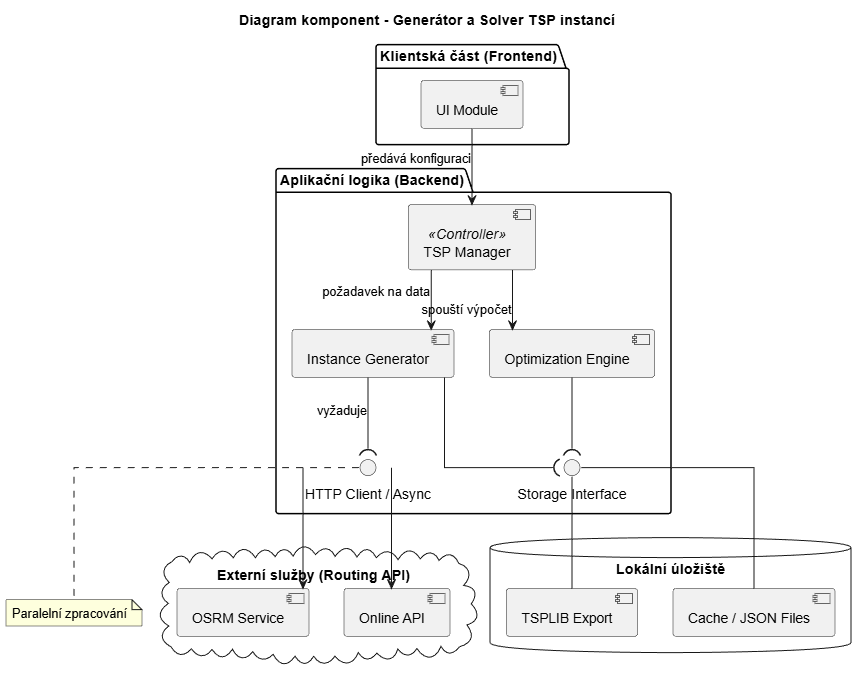
\includegraphics[width=\textwidth]{Figures/component_diagram.png}
    \caption{Diagram komponent}
    \label{fig:component_diagram}
\end{figure}

Diagram komponent \ref{fig:component_diagram} znázorňuje modulární strukturu systému. Centrálním bodem je \textit{TSP Manager}, který koordinuje tok dat mezi uživatelským rozhraním, tvorbou matice a optimalizačním jádrem. Ve výsledné implementaci není samostatný runtime modul \textit{Instance Generator}; jeho původně navržené odpovědnosti jsou rozděleny mezi komponenty rozhraní, routovací vrstvu a I/O strategie. Výpočetní jádro \textit{Optimization Engine} je odděleno od síťové vrstvy, takže lze měnit optimalizační metody bez zásahu do routovacích volání.

\subsection{Aktivitní diagram}
Popisuje generování instance od vstupu až po finální export s pomocí externího API. Podobně lze přistupovat i k lokálnímu OSRM modelu.
\begin{figure}[H]
    \centering
    
\includegraphics[width=0.78\textwidth,height=0.58\textheight,keepaspectratio]{Figures/TSP_gen_activity_diagram.png}
    \caption{Diagram aktivit v aplikaci}
    \label{fig:activity_diagram}
\end{figure}

Výpočet matice vzdáleností pro trasové metriky využívá dávkové volání maticových rozhraní služeb ORS a OSRM. Počet vyhodnocovaných dvojic je $n^2-n$, ale v praxi se neřeší samostatným dotazem pro každou dvojici; matice je sestavována po blocích. Paralelní sekce v diagramu (\ref{fig:activity_diagram}) proto reprezentuje neblokující obsluhu síťových operací a následné skládání dílčích výsledků. Celková doba je ovlivněna latencí, limity služeb i lokálním zpracováním dat.

\subsection{Třídní diagram}
Diagram tříd \ref{fig:class_diagram}. Znázorňuje statickou strukturu navrženého systému. Architektura je striktně rozdělena do několika logických celků, které zajišťují oddělení odpovědnosti a rozšiřitelnost.
\textbf{Klíčové komponenty a jejich vazby:}

\begin{itemize}
    \item \textbf{Řídicí vrstva:} Centrálním bodem je třída \texttt{TSPManager}. Zajišťuje validaci vstupu, volbu metriky, sestavení matice a spuštění optimalizační metody
    \item \textbf{Optimalizační jádro:} Třída \texttt{OptimizationEngine} mapuje zvolený algoritmus na konkrétní implementační funkci. To umožňuje jednotné volání více metod nad stejnou maticí
    \item \textbf{Stav aplikace a notifikace:} Sdílený stav je soustředěn ve třídě \texttt{AppState}. Synchronizace mezi panely rozhraní a mapou je realizována oznamovacím mechanismem, návrhovým vzorem Observer
    \item \textbf{Import a export:} Vrstva I/O používá strategii formátů (\texttt{TspGeoStrategy}, \texttt{TspEuc2DStrategy}, \texttt{GpxStrategy}), čímž odděluje orchestraci od konkrétní serializace dat
\end{itemize}



\section{Návrh architektury}
Systém je navržen s důrazem na oddělení odpovědností jednotlivých vrstev.

\subsection{Použité návrhové vzory}
Z hlediska softwarového inženýrství je systém navržen s využitím osvědčených návrhových vzorů, které zajišťují modularitu systému:

\begin{itemize}
    \item \textbf{Strategy:} Použita ve vrstvě I/O, kde každá strategie řeší konkrétní formát souboru bez změny orchestrace
    \item \textbf{Observer:} Stav aplikace rozesílá změny odběratelům, takže se uživatelské rozhraní i mapa aktualizují konzistentně z jednoho zdroje pravdy
    \item \textbf{Responsibility-Driven Design:} Optimalizační jádro využívá mapování parametrů na algoritmy i metriky
\end{itemize}

\subsection{Modulární struktura}
\begin{itemize}
    \item \textbf{Core modul:} Řídí životní cyklus výpočtu, validaci vstupu a spuštění optimalizace
    \item \textbf{Routovací vrstva:} Realizuje volání ORS a OSRM, skládání matic po blocích a náhradní režim při chybách služby
    \item \textbf{I/O vrstva:} Zajišťuje import a export TSPLIB a GPX prostřednictvím strategií formátů
    \item \textbf{Prezentační vrstva:} Kombinuje mapové zobrazení v \texttt{QWebEngineView} s ovládacími panely PyQt6
\end{itemize}

\section{Návrh datového modelu}
Základním objektem systému je \texttt{TSPInstance}, která vnitřně reprezentuje graf $G=(V, E)$.

\subsection{Datové struktury}
V paměti bude instance uložena jako objekt obsahující:
\begin{itemize}
    \item \texttt{nodes}: Seznam objektů (ID, název, lat, lon).
    \item \texttt{distance\_matrix}: Dvourozměrné pole $n \times n$.
    \item \texttt{metadata}: Informace o zdroji dat, typu dopravy a datu vytvoření.
\end{itemize}

\section{Design paralelního zpracování datových požadavků}
\label{sec:design_paralelizace}

Klíčovou výzvou při generování reálných TSP instancí je efektivní získávání dat z externích služeb. Proces sestavení matice vzdáleností pro $n$ lokalit vyžaduje $n(n-1)$ dotazů na nalezení nejkratší cesty. Vzhledem k povaze této úlohy je proces klasifikován jako \textit{I/O bound} operace, kde hlavním limitujícím faktorem není výpočetní výkon procesoru (CPU), ale latence síťové komunikace a propustnost API.

\subsection{Analýza úzkého hrdla při komunikaci s mapovými API}
Při sekvenčním přístupu k API dochází k výraznému nevyužití systémových zdrojů, neboť CPU většinu času nečinně čeká na doručení HTTP odpovědi. 
Pokud uvažujeme průměrnou latenci jednoho požadavku $t_{lat} = 100$\,ms, pak pro instanci o velikosti $n=100$ (10\,000 tras) činí celkový čas generování:
\begin{equation}
T_{total} = n(n-1) \cdot t_{lat} \approx 10\,000 \cdot 0,1\,\text{s} = 1\,000\,\text{s} \approx 16,7\,\text{min}.
\end{equation}
Tato hodnota je pro interaktivní nástroj neakceptovatelná. Nasazení paralelního zpracování umožňuje odbavovat více požadavků současně, čímž se celková doba výrazně zkracuje. Výsledné zrychlení je však dáno kombinací latence, propustnosti sítě, omezení poskytovatele služby a lokálního zpracování odpovědí.

\subsection{Model neblokujícího získávání matic vzdáleností}
Pro řešení výše zmíněného problému je v aplikaci použito neblokující zpracování síťových operací. V praxi jde o kombinaci dávkového volání maticových rozhraní a přesunu síťově náročných částí mimo hlavní vlákno grafického rozhraní.

\begin{itemize}
    \item \textbf{Dávkování požadavků:} Kvůli limitům maticového rozhraní jsou dvojice zdroj - cíl rozděleny do bloků, které se postupně skládají do výsledné matice
    \item \textbf{Náhradní režim:} Při chybě ORS volání se systém přepne na lokální OSRM a při selhání obou trasových služeb použije bodovou metriku
\end{itemize}

\subsection{Sekvenční diagram získávání dat}
Sekvenční diagram komunikace mezi frontendem, backendem (generátorem) a API je z důvodu čitelnosti uveden v příloze na obrázku~\ref{fig:sequence_diagram}. Ilustruje, že generátor nečeká na dokončení prvního požadavku, ale v rychlém sledu odesílá další, přičemž odpovědi zpracovává v pořadí, v jakém přicházejí ze sítě.

\subsection{Návrh mezipaměti pro redukci duplicitních dotazů}
Vzhledem k limitům veřejných služeb je důležitou částí návrhu mezipaměť geokódování. 

\begin{enumerate}
    \item \textbf{Identifikace dotazů:} Geokódovací požadavky jsou ukládány podle textového vstupu a profilu služby.
    \item \textbf{Perzistence:} Data jsou ukládána v lokálním souboru, takže opakované dotazy na stejné lokality nevyvolávají nové síťové volání.
    \item \textbf{Asymetrie tras:} Směr $A \to B$ a $B \to A$ je při výpočtu matic vyhodnocován odděleně, protože v silniční síti obecně neplatí symetrie.
\end{enumerate}


\section{Volba technologií}
Pro implementaci byly zvoleny technologie s ohledem na efektivitu vývoje a dostupnost vědeckých knihoven.

\begin{itemize}
    \item \textbf{Programovací jazyk:} Python 3.13
    \item \textbf{Komunikace po síti:} knihovna \texttt{requests} a síťové komponenty Qt (\texttt{QNetworkAccessManager}) pro routovací i geokódovací volání
    \item \textbf{Zpracování dat:} standardní datové struktury jazyka Python a specializované pomocné funkce pro práci s maticemi vzdáleností
    \item \textbf{Mapové podklady:} Leaflet vykreslovaný v \texttt{QWebEngineView} nad daty OpenStreetMap
    \item \textbf{Mapová API:}
    \begin{itemize}
        \item \textbf{OpenRouteService:} Primární zdroj trasových matic i geokódovacích služeb
        \item \textbf{OSRM (Open Source Routing Machine):} Lokální náhradní zdroj pro výpočet matic a tras při výpadku primární služby
    \end{itemize}
    \item \textbf{Volba oproti rozhraní Mapy.cz:} Po předchozí domluvě s vedoucím práce bylo pro tuto implementaci zvoleno API OpenRouteService (ORS): služba je pro běžné a akademické využití při vlastním API klíči bezplatná, má otevřený ekosystém a veřejnou dokumentaci, klíč lze získat v řádu minut a limity dotazů jsou pro účely práce přijatelné. ORS navíc poskytuje přehledné příklady volání endpointů včetně maticových a directions rozhraní, která odpovídají potřebě generátoru.
\end{itemize}
\endinput